\documentclass{standalone}

\usepackage{pgfplots}

\begin{document}
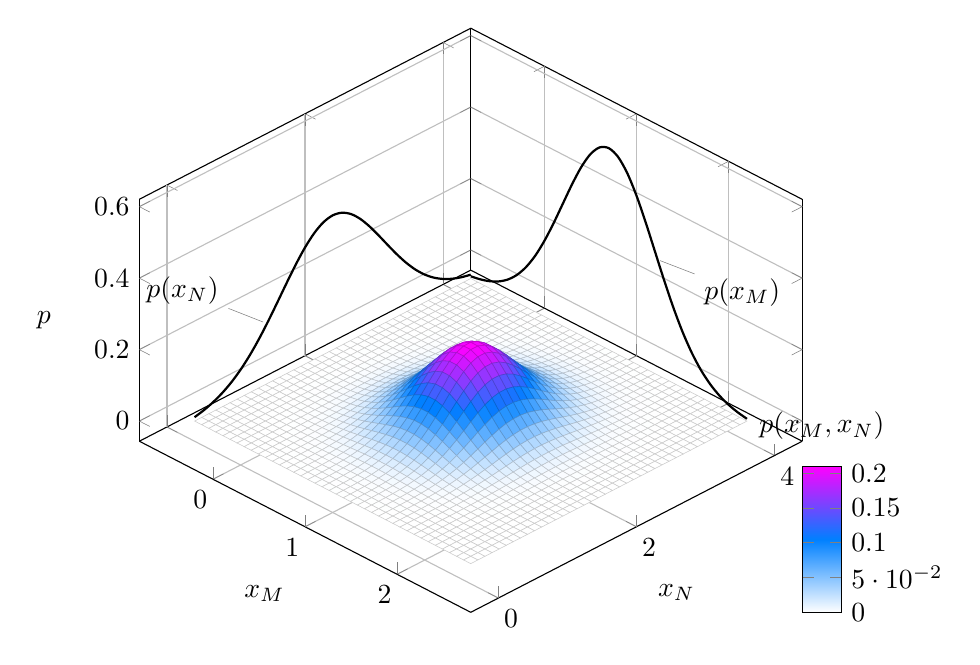
\begin{tikzpicture}[
    declare function={mu1=1;},
    declare function={mu2=2;},
    declare function={sigma1=0.5;},
    declare function={sigma2=0.75;},
    declare function={normal(\m,\s)=1/(2*\s*sqrt(pi))*exp(-(x-\m)^2/(2*\s^2));},
    declare function={bivar(\ma,\sa,\mb,\sb)=
        1/(2*pi*\sa*\sb) * exp(-((x-\ma)^2/\sa^2 + (y-\mb)^2/\sb^2))/2;}]
    \pgfplotsset{colormap={cool}{rgb255(0cm)=(255,255,255); rgb255(1cm)=(0,128,255); rgb255(2cm)=(255,0,255)}}%
\begin{axis}[
    colormap name=cool,
    width=10cm, height=9cm,
    view={45}{45},
    enlarge x limits,
    enlarge y limits,
    grid=major,
    domain=-0.5:2.5,
    y domain=0:4,
    ymin=0,
    ymax=4,
    xmin=-0.5,
    xmax=2.5,
    samples=40,
    xlabel=$x_M$,
    ylabel=$x_N$,
    zlabel={$p$},
    every axis z label/.style={rotate=0, at={(current axis.west)}, left=10mm},
    colorbar,
    colorbar style={
        at={(1,0)},
        anchor=south west,
        height=0.25*\pgfkeysvalueof{/pgfplots/parent axis height},
        title={$p(x_M,x_N)$}
    }
]
\addplot3 [surf, shader=faceted, very thin] {bivar(mu1,sigma1,mu2,sigma2)};
\addplot3 [domain=-0.5:2.5,samples=31, samples y=0, thick, smooth] (x,4,{normal(mu1,sigma1)});
\addplot3 [domain=0:4,samples=31, samples y=0, thick, smooth] (-0.5,x,{normal(mu2,sigma2)});
% \addplot3 [domain=0:4,samples=31, samples y=0, thick, smooth] (x,2,{normal(mu1,0.95)});
\node at (axis cs:-0.4,1,0.18) [pin=165:$p(x_N)$] {};
\node at (axis cs:1.45,4,0.32) [pin=-15:$p(x_M)$] {};
\end{axis}
\end{tikzpicture}
\end{document}